
\section{Targets}
\label{sec:targets}

\begin{figure}[H]
    \hspace*{-2.5cm}
    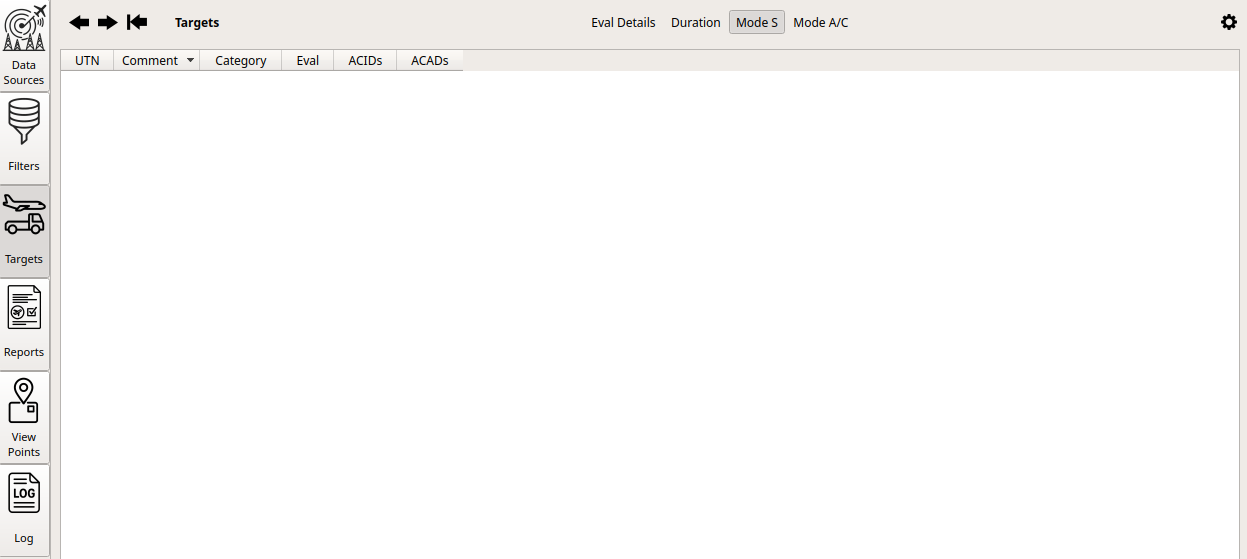
\includegraphics[width=19cm,frame]{figures/ui_targets.png}
  \caption{Targets Overview}
\end{figure}

In the 'Targets' tool, all existing unique targets are listed. If no reference data has been reconstructed, and thus no associations were calculated, the list is empty. 
See chapter \nameref{sec:reconst} for instructions about how to reconstruct reference data. \\

The table listing the targets obtains mutliple columns, which are divided into groups.
These groups can be hidden or shown individually for more clarity. The following groups and columns exist:

\begin{itemize}  
\item Base Items: These columns are always visible
\begin{itemize}  
  \item UTN: Unique Target Number
  \item Comment: A comment which can be set by the user \hl{TODO?}
  \item Category: The target's emitter category \hl{TODO?}
  \item Eval: An icon showing the target's Evaluation usage status
\end{itemize}
\item Eval Details: Columns showing details for Evaluation \hl{TODO?}
\begin{itemize}  
  \item Eval Excluded: \hl{TODO}
\end{itemize}
\item Duration: Columns showing details about the target's duration
\begin{itemize}  
  \item \#Updates: Sum number of target reports 
  \item Begin: First timestamp of UTN
  \item End: Last timestamp of UTN
  \item Duration: Duration in HH:MM:SS.SSS
\end{itemize}
\item Mode S: Columns regarding the target's Mode S attributes
\begin{itemize}  
  \item ACIDs: Target identification(s)
  \item ACADs: Target addresses (hexadecimal)
\end{itemize}
\item Mode A/C: Columns regarding the target's Mode A/C attributes
\begin{itemize}  
  \item M3/A: Mode 3/A code(s) (octal)
  \item MC Min: Mode C code minimum [ft]
  \item MC Max: Mode C code maximum [ft]
\end{itemize}
\end{itemize}
\ \\

\hl{TODO} Check table \\

The individual groups can be enabled/disabled by clicking the group buttons above the target list. \\

After running the Reconstruct References task, the table can look as follows:

\begin{figure}[H]
  \hspace*{-2cm}
    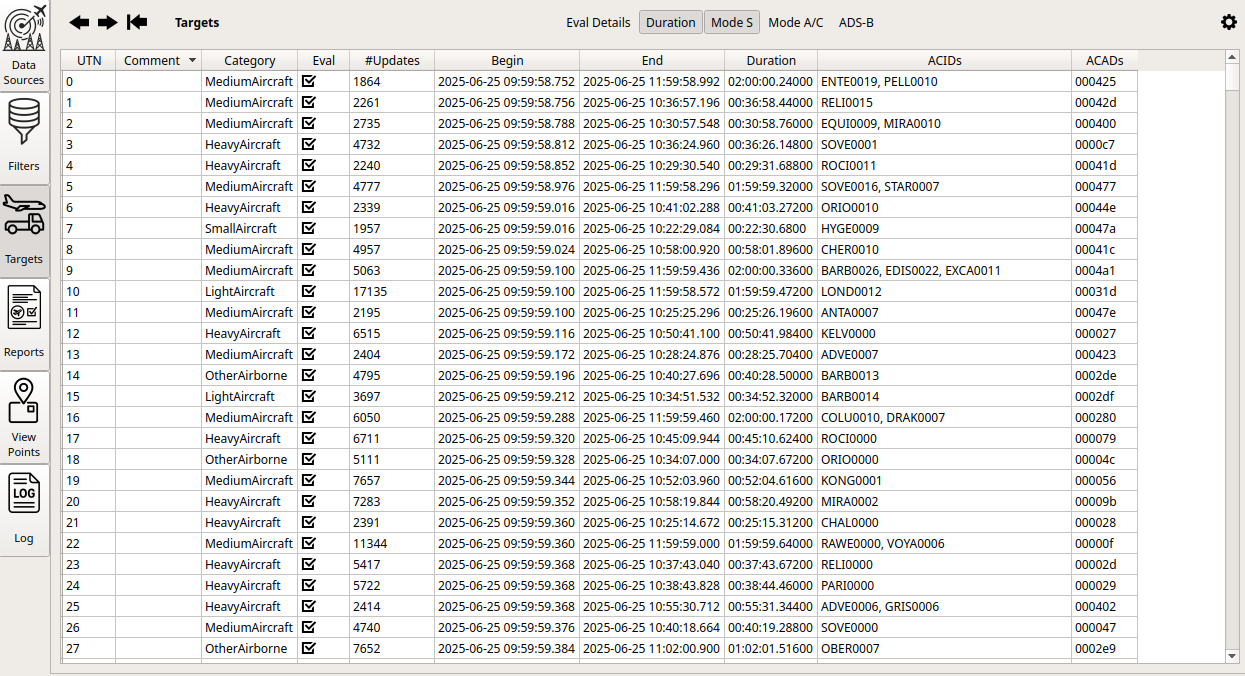
\includegraphics[width=18cm,frame]{figures/ui_targets2.png}
  \caption{Targets Tab with reconstructed unique targets}
\end{figure}

When clicking a target, all data associated to the respective target is loaded. The Targets tab is useful for inspecting the association results, 
removing certain targets from Evaluation and inspecting already removed ones. \\

Single rows can be selected by clicking on them which triggers a loading process showing this exact target(s) (with all associated data) in the available Views. 
Multiple targets can be selected using the shift key (range selection) or control key (add/remove single targets).

\begin{figure}[H]
  \hspace*{-2cm}
    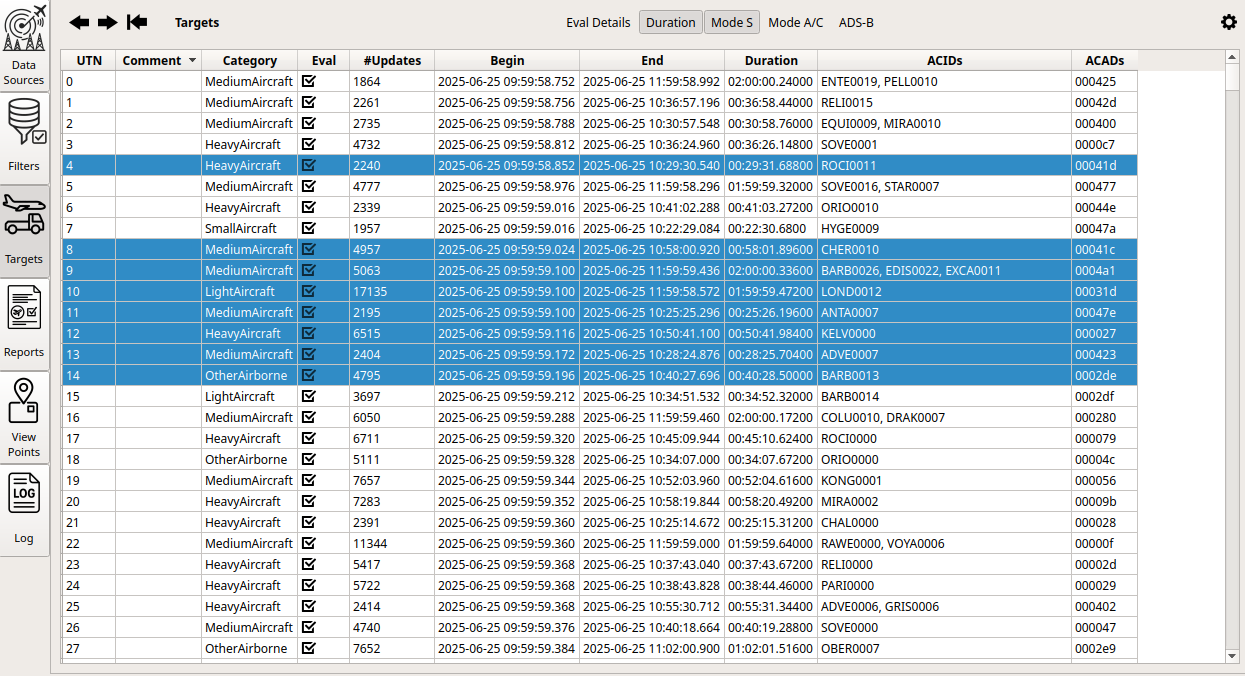
\includegraphics[width=18cm,frame]{figures/ui_targets3.png}
  \caption{Targets Tab with multiple selected targets}
\end{figure}

When clicking on a column header, the ordering of the target table can be changed, e.g. to find:

\begin{itemize}  
\item Targets with short duration
\item Missing certain identification attributes
\item Minimum or maximum Mode C code
\end{itemize}
\ \\

Such targets can then be loaded by selecting a range of targets using the shift key - e.g. all with a duration shorter than a certain value of interest. \\

Please \textbf{note} that the target information (including Evaluation usage and comments) are persisted in the database. \\

The \includegraphics[width=0.5cm,frame]{../../data/icons/edit.png} button in the top right corner can be used to execute several actions.
Clicking the button opens the following menu.

\begin{figure}[H]
    \center
    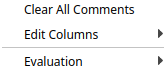
\includegraphics[width=6cm,frame]{figures/ui_targets_config.png}
  %\caption{Data Sources Overview}
\end{figure}

\begin{itemize}
  \item Clear All Comments: Clears the comments of all targets
  \item Edit Columns: Shows/hides column groups (alternatively to pressing the group buttons)
  \item Evaluation: Operations for setting Evaluation target usage and constraints globally for all targets, see \nameref{sec:ui_eval_usage}
 \end{itemize} 
 \  \\

\subsection{Evaluation Usage and Constraints}
\label{sec:ui_eval_usage}

\hl{TODO: Describe usage and constraints principle, describe single target operations} \\

The 'Evaluation' submenu provides global operations for settings Evaluation target usage and constraints for all listed targets.

\begin{figure}[H]
  \center
  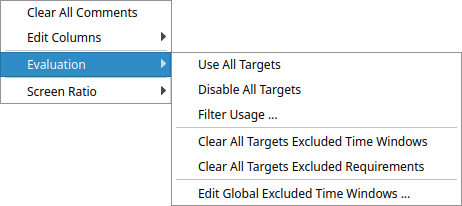
\includegraphics[width=6cm,frame]{figures/ui_targets_config_eval.png}
%\caption{Data Sources Overview}
\end{figure}

\begin{itemize}
  \item Use All Targets: Enable all targets for usage in Evaluation
  \item Disable All Targets: Disable all targets for usage in Evaluation
  \item Filter Usage: Filter targets for usage in Evaluation, see \nameref{sec:ui_target_filtering}
  \item Clear All Targets Excluded Time Windows: Clear the specified Evaluation exclusion time windows of all targets
  \item Clear All Targets Excluded Requirements: Clear the specified excluded Evaluation requirements of all targets
  \item Edit Global Excluded Time Windows
\end{itemize} 
\ \\

\hl{TODO: Describe global target operations listed above} \\

Please \textbf{note} that Evaluation usage and constraints of the targets can also be configured after an Evaluation has been run.
This will mark all existing Evaluation Reports as outdated, these can be refreshed afterwards to adapt to the target changes.
See chapter \nameref{sec:eval} for details.

\subsection{Target Filtering}
\label{sec:ui_target_filtering}

Using the \includegraphics[width=0.5cm,frame]{../../data/icons/edit.png} button and selecting \textit{Evaluation $\rightarrow$ Filter Usage} opens a dialog, 
which can be used to dynamically filter UTNs for Evaluation usage based on specified values.

\begin{figure}[H]
    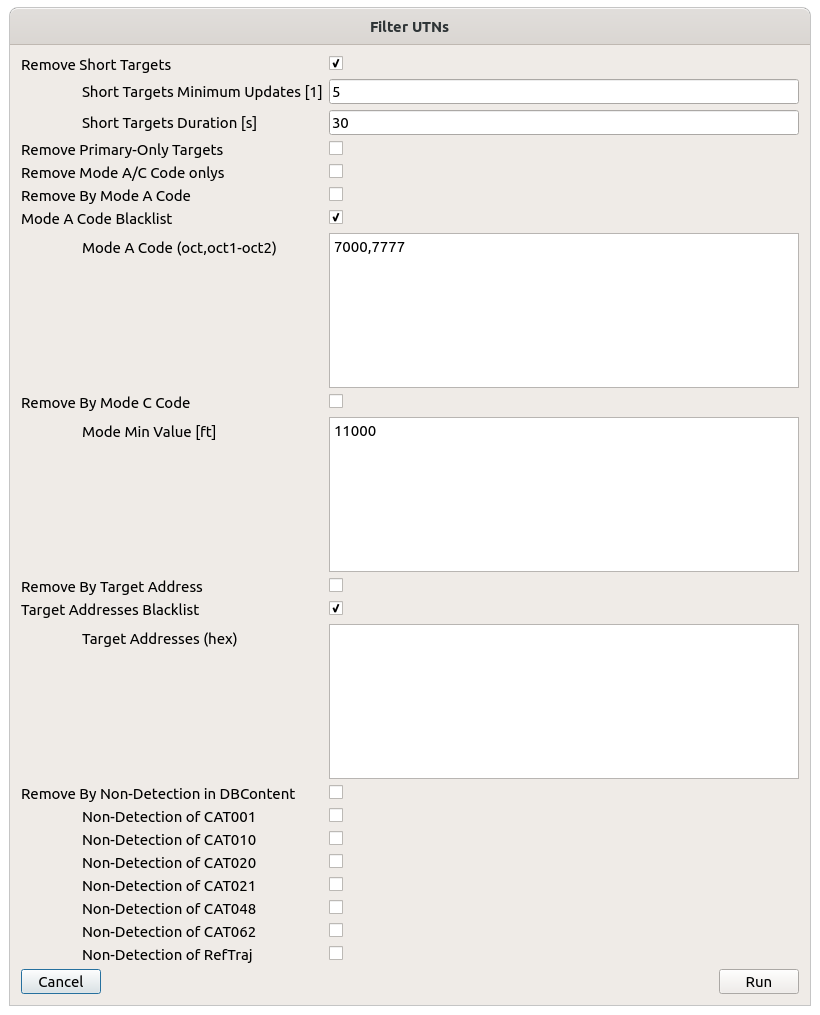
\includegraphics[width=15cm]{figures/filter_utns.png}
  \caption{Targets Filter UTNs dialog}
\end{figure}

\begin{itemize}  
\item Remove Short Targets: Removes targets with a small number of target reports or duration
\item Remove Primary-Only Targets: Removes primary-only targets (w/o secondary attributes)
\item Remove Mode A/C Code onlys: Removes targets without Mode S attributes
\item Remove by Mode A Code: Removes targets having a Mode A code given in the list
\item Mode A Code Blacklist: Whether the Mode A codes should be used as blacklist or whitelist
\item Remove by Mode C Code: Removes targets having a Mode C code smaller than the given value
\item Remove by Target Address: Removes targets having a Mode S target address given in the list
\item Target Address Blacklist: Whether the Target Addresses should be used as blacklist or whitelist
\item Remove by Non-Detection of DBContent: Removes targets not being detected by a given DBContent
\end{itemize}
\ \\

When the 'Run' button is clicked, all (enabled) targets are checked and are disabled if any of the selected filters apply.
A comment will be set for each disabled target, describing the reason for its removal.

\begin{figure}[H]
  \hspace*{-2cm}
    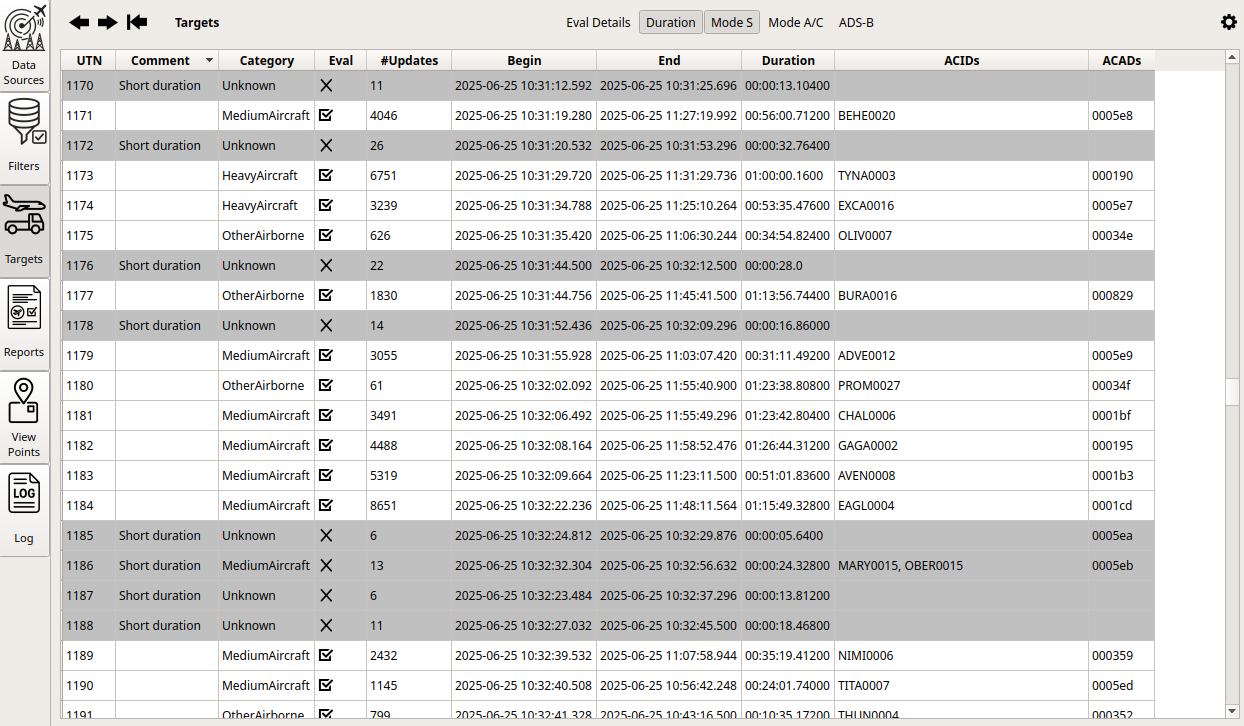
\includegraphics[width=18cm,frame]{figures/filter_utns_done.png}
  \caption{Targets Tab after UTN Filtering}
\end{figure}
